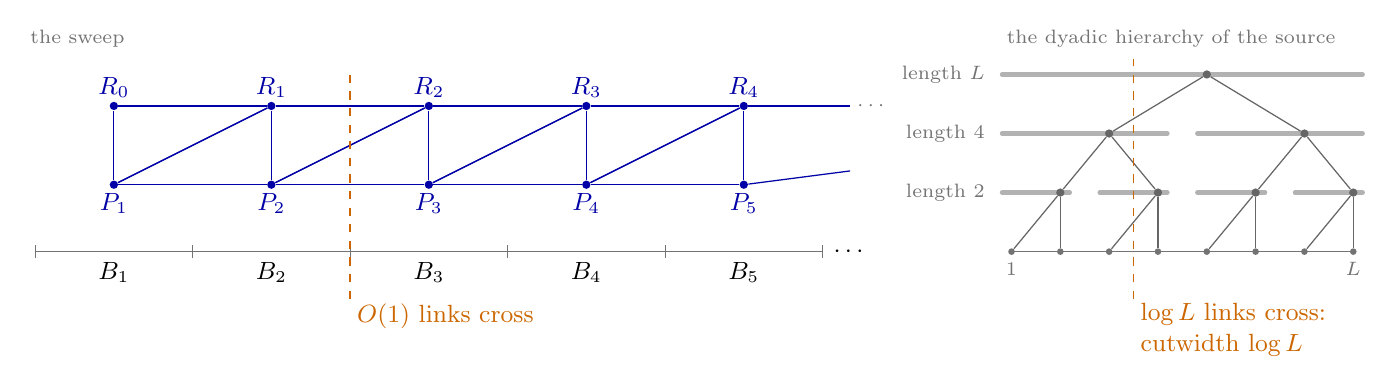
\begin{tikzpicture}[x=1cm, y=1cm, line width=0.3pt,
    lab/.style={font=\small, inner sep=1pt},
    annot/.style={font=\scriptsize, text=black!55, inner sep=1pt},
    party/.style={circle, fill=blue!65!black, inner sep=0pt, minimum size=3pt},
    link/.style={draw=blue!65!black, line width=0.45pt},
    site/.style={circle, fill=black!55, inner sep=0pt, minimum size=2.4pt},
    dnode/.style={circle, fill=black!60, inner sep=0pt, minimum size=3pt},
    dlink/.style={draw=black!60, line width=0.45pt},
    bar/.style={draw=black!30, line width=1.6pt, line cap=round},
    cut/.style={dashed, color=orange!80!black, line width=0.5pt}]
  \def\b{2.0}\def\yP{0.85}\def\yR{1.85}
  \node[annot, anchor=south west] at (-0.1, 2.55) {the sweep};
  \draw[black!55] (0, 0) -- (5*\b, 0);
  \foreach \i in {0,...,5} { \draw[black!55] (\i*\b, 0.08) -- (\i*\b, -0.08); }
  \foreach \i in {1,...,5} {
    \node[lab, anchor=north] at ({(\i-0.5)*\b}, -0.1) {\(B_{\i}\)};
  }
  \node[lab, anchor=west] at (5*\b + 0.1, 0) {\(\cdots\)};
  \foreach \i in {1,...,5} {
    \node[party] (P\i) at ({(\i-0.5)*\b}, \yP) {};
    \node[lab, anchor=north, text=blue!65!black] at ({(\i-0.5)*\b}, \yP-0.07) {\(P_{\i}\)};
  }
  \foreach \k in {0,...,4} {
    \pgfmathtruncatemacro{\j}{\k+1}
    \node[party] (R\k) at ({(\j-0.5)*\b}, \yR) {};
    \node[lab, anchor=south, text=blue!65!black] at ({(\j-0.5)*\b}, \yR+0.07) {\(R_{\k}\)};
  }
  \draw[link] (P1) -- (R0);
  \draw[link] (R0) -- (R1);
  \draw[link] (P1) -- (R1);
  \foreach \k in {1,...,4} {
    \pgfmathtruncatemacro{\j}{\k+1}
    \draw[link] (P\k) -- (R\k);
    \draw[link] (P\j) -- (R\k);
    \draw[link] (P\k) -- (P\j);
    \ifnum\k<4
      \draw[link] (R\k) -- (R\j);
      \draw[link] (P\j) -- (R\j);
    \fi
  }
  \draw[link] (R4) -- (5*\b + 0.35, \yR);
  \draw[link] (P5) -- (5*\b + 0.35, {\yP + 0.5*(\yR-\yP)*0.35/\b*2});
  \node[annot, anchor=west] at (5*\b + 0.4, \yR) {\(\cdots\)};
  \draw[cut] (2*\b, -0.6) -- (2*\b, 2.3);
  \node[lab, anchor=north west, text=orange!80!black] at (2*\b + 0.05, -0.62) {\(O(1)\) links cross};
  \begin{scope}[xshift=12.4cm]
    \def\s{0.62}\def\h{0.75}
    \node[annot, anchor=south west] at (-0.1, 2.55) {the dyadic hierarchy of the source};
    \draw[black!55] (0, 0) -- (7*\s, 0);
    \foreach \i in {1,...,8} {
      \node[site] (S\i) at ({(\i-1)*\s}, 0) {};
    }
    \node[annot, anchor=north] at (0, -0.1) {\(1\)};
    \node[annot, anchor=north] at (7*\s, -0.1) {\(L\)};
    \foreach \a/\c/\p in {1/2/2, 3/4/4, 5/6/6, 7/8/8} {
      \draw[bar] ({(\a-1)*\s - 0.12}, \h) -- ({(\c-1)*\s + 0.12}, \h);
      \node[dnode] (D\a\c) at ({(\p-1)*\s}, \h) {};
      \draw[dlink] (D\a\c) -- (S\a);
      \draw[dlink] (D\a\c) -- (S\c);
    }
    \foreach \a/\m/\n/\c/\p in {1/2/3/4/3, 5/6/7/8/7} {
      \draw[bar] ({(\a-1)*\s - 0.12}, 2*\h) -- ({(\c-1)*\s + 0.12}, 2*\h);
      \node[dnode] (D\a\c) at ({(\p-1)*\s}, 2*\h) {};
      \draw[dlink] (D\a\c) -- (D\a\m);
      \draw[dlink] (D\a\c) -- (D\n\c);
    }
    \draw[bar] (-0.12, 3*\h) -- (7*\s + 0.12, 3*\h);
    \node[dnode] (D18) at (4*\s, 3*\h) {};
    \draw[dlink] (D18) -- (D14);
    \draw[dlink] (D18) -- (D58);
    \node[annot, anchor=east] at (-0.3, \h) {length \(2\)};
    \node[annot, anchor=east] at (-0.3, 2*\h) {length \(4\)};
    \node[annot, anchor=east] at (-0.3, 3*\h) {length \(L\)};
    \draw[cut] (2.5*\s, -0.6) -- (2.5*\s, 2.45);
    \node[lab, anchor=north west, text=orange!80!black, align=left] at (2.5*\s + 0.05, -0.62)
      {\(\log L\) links cross:\\ cutwidth \(\log L\)};
  \end{scope}
\end{tikzpicture}
